\section{Implementation}\label{result}

This chapter serves as a documentation of the resulting code when following the porting methodology specified in the previous chapter. This is accomplished by showing the step-by-step process of how the porting of a function was accomplished. The functionality chosen as an example throughout this chapter is the concatenation of two separate lists into one. For each step in the process a sample implementation of the concatenation operator is presented. This choice was made since it is one of the less trivial functions of the original C code, providing a better foundation for the reader to get a grasp of how the porting process was applied. The complete implementation result can be seen at the project's GitHub repository \cite{LINKEDLISTREPO}.

\subsection{Environment}

The first step in the process was to isolate the files needed by the data structure so that they could be executed outside the context of the FreeBSD codebase. As the linked list code chosen was in the lower levels of the operating system, this was an elementary process since there few dependencies needed to be included. However, some FreeBSD specific OS-level definitions which were not present in the Linux standard library needed to be included. This complicated the process somewhat but was solved by including these into the queue source.

The linked list source code was fully made up of macros; predefined text snippets that are expanded into code during the pre-processing stage of compilation. This meant that the macros needed to be expanded into valid C code so that coverage of any tests could be measured. This was done by using the GCC compiler and the -E flag \cite{gcc_man}. However, using this method when expanding code directly would yield no output since macros are expanded where they are used, not where they are defined. Therefore, a level of indirection was added by defining proxy functions using the macros which as well as expanding the text into valid C code enabled the coverage of this code to be measured. The added indirection somewhat changed the semantics of how the library was invoked by introducing function calls that would otherwise not be present. Defining these functions as inline could make it so that the resulting compiler output was identical, or very close to the one generated using the macros directly.
    

\subsection{Behavioral Properties}

The source code of the concatenation function (see figure \ref{fig:concat}) shows that the function takes two lists as arguments named \textit{head1} and \textit{head2} (line 2 and 3). The argument names come from the fact that the first node of a list is referred to and stored in a head structure but will, where appropriate, be referred to as lists. The function concatenates the two lists into one where the head of the first list becomes the head of the concatenated, and the second lists head is set to be the next element to the tail of the first list. This indicates that the tail of the second list becomes the tail of the concatenated list.
\begin{figure}[H]
 \vspace{12pt}
\begin{lstlisting}[style=CSTYLE, belowskip=1pt]
void SLIST_CONCAT_impl(
    mySinglyLinkedListHead* head1, 
    mySinglyLinkedListHead* head2){
    IntegerSLISTEntry *curelm = head1->slh_first;
    if (curelm == NULL) {                                    
        if ((head1->slh_first = head2->slh_first) != NULL) {
            head2->slh_first = NULL;                                   
        }
    } else if (head2->slh_first != NULL) {               
        while (curelm->entries.sle_next != NULL){  
            curelm = curelm->entries.sle_next;         
        }                                                                                                              
        curelm->entries.sle_next = head2->slh_first
        head2->slh_first = NULL
    }
}
\end{lstlisting}
    \caption{The Concatenate Function}
    \label{fig:concat}
\end{figure}
The concatenation is accomplished by first checking if the first list - the \textit{head1} pointer argument - is populated by any nodes (line 5). If that is the case, it assigns the head of the second list, the \textit{head2} pointer argument, to the address of the first. This is done while in the same statement checking if the second list is populated (line 6). If it is, it sets the second list to be empty to avoid duplicate references (line 7). 
In the case of the first list being populated, the function checks in the else if clause if the second list is populated as well (line 9). If it is, then the function iterates through the first list to reach its tail element (lines 10 to 12). The head of the second list then becomes the next element of the tail element in the first list (line 13). This makes the second list appended to the first i.e., they are now concatenated. As a last statement is the head of the second list set to NULL (line 14). This shows that the function not only "copies" \textit{head2} onto \textit{head1}, but "moves" the second list onto the end of the first.

When describing the valid states and functions of the program, a hypothesis about a certain function was deduced from the code using the previously mentioned Hoare logic (see section \ref{implproc}). This means that for each function of the target source code were a set of pre- and post-conditions identified. Each precondition needed to identify valid initial states on which the function could be applied, and each post-condition needed to be a statement about the resulting state of the list that should be true after the execution of the function. To form a behavioral understanding on the preconditions of the concatenate function, it can be stated that the function takes two lists as arguments. This allows the conclusion that the precondition can be based on the following four situations:

\begin{itemize}
  \item Both lists are empty
  \item The first list is populated and the second is empty
  \item The first list is empty and the second is populated
  \item Both lists are populated
\end{itemize}

These four situations form the foundation for these following behavioral statements where the first one is when both lists are empty. In \ref{fig:prop1} and forward, the list variables are prepended with P or R - corresponding to the Hoare logic (see section \ref{implproc}) - indicating whether they are the values before or after the operation (see figure \ref{fig:prop1}). The \textit{isEmpty} helper function indicates whether a list is empty, and the behavioral reasoning states that if both lists are empty, the test needs to check that both lists still are empty after the concatenation procedure. 

\begin{figure}[H]
 \vspace{12pt}
\begin{verbatim}
       Precondition: isEmpty(P_list1) AND isEmpty(P_list2)
    
       Function: concatenate(P_list1, P_list2)
    
       Postcondition: isEmpty(R_list1) AND isEmpty(R_list2)
\end{verbatim}
    \caption{Properties of Concatenation Operation 1}
    \label{fig:prop1}
\end{figure}


Following this stipulation, it can be stated that the two cases where only one list is populated results in the same end state. This forms the behavioral basis seen in figure \ref{fig:prop2}. The \textit{validList} helper function checks that a list is valid, \textit{size} returns the number of elements in the list and \textit{first} and \textit{last} return the first and the last element of a list.

\begin{figure}[H]
\begin{verbatim}
       Precondition: 
           • case1 -> validList(P_list1) AND isEmpty(P_list2)
           • case2 -> isEmpty(P_list1) AND validList(P_list2)
        
       Function: concatenate(P_list1, P_list2)
    
       Postcondition:
           • case1 -> isEmpty(R_list2) AND
                      first(R_list1) = first(P_list1) AND
                      last(R_list1) = last(P_list1) AND 
                      size(R_list1) = size(P_list1)
           • case2 -> isEmpty(R_list2) AND
                      first(R_list1) = first(P_list2) AND
                      last(R_list1) = last(P_list2) AND
                      size(R_list1) = size(P_list2)
\end{verbatim}
    \caption{Properties of Concatenation Operation 2}
    \label{fig:prop2}
\end{figure}


This basis indicates that the tests need to assert that the head of the first element of the populated list in the precondition always is returned being assigned to the element of the first list in the post-condition. It must as well assert that the last element of the populated list becomes the last element of the concatenated list. The tests must also assert that the second list in the post-condition always is empty, and that the length of the concatenated list always is of the same length as the initially populated one. 

If both lists are populated the behavioral basis becomes more complicated since several more assertions can be made on the post-condition (see figure \ref{fig:prop3}). 
\begin{figure}[H]
\begin{nonbreaking}
\begin{verbatim}
       Precondition: validlist(P_list1) AND validList(P_list2)
    
       Function: concatenate(P_list1, P_list2)
    
       Postcondition: first(R_list1) = first(P_list1) AND
                      last(R_list1) = last(P_list2) AND
                      size(R_list1) = 
                      (size(P_list1)+size(P_list2)) AND
                      isEmpty(R_list2) AND
                      {P_list1} SUBSETOF {R_list1} AND 
                      {P_list2} SUBSETOF {R_list1}
     
\end{verbatim}
\end{nonbreaking}
    \caption{Properties of Concatenation Operation 3}
    \label{fig:prop3}
\end{figure}


This behavioral basis states that in the case of both lists being populated, the head of the concatenated list must always be the head of the first list in the precondition. The basis also indicates that the tail of the second list always becomes the tail of the concatenated list. Since the lists are being concatenated the size of the concatenated list must also always match the sum of the size of both initial lists. This also means that the size of the second list always must be zero as a post condition i.e., the second list becomes empty. Lastly it states that the nodes of the two initial lists must always be a subset of the concatenated list.

\subsection{Tests}

To verify that the actual behavior conformed to the behavioral basis, tests were written asserting that this is the case. Both unit and stateful property-based tests were written in \textit{GoogleTest} combined with \textit{RapidCheck}. An example of a testing property for the concatenate function takes vectors of integer values (see lines 3 and 4 figure \ref{fig:size}) generated by \textit{RapidCheck} and converts them into two separate lists of the \textit{mySinglyLinkedList} type through the helper function \textit{createList} (lines 6 through 9). These vectors were of an arbitrary number of elements, including empty. 

\begin{figure}[H]
 \vspace{12pt}
\begin{lstlisting}[style=CSTYLE] 
RC_GTEST_PROP(SLIST, 
concatenatingListsYieldsCorrectSizeOnList1, 
(std::vector<IntegerSLISTEntry> a,
std::vector<IntegerSLISTEntry> b)){

    mySinglyLinkedListHead headA{nullptr};
    createList(headA, a);
    mySinglyLinkedListHead headB{nullptr};
    createList(headB, b);
    unsigned int expectedSize = a.size() + b.size();
    
    SLIST_CONCAT_impl(&headA, &headB);
    
    IntegerSLISTEntry *entry;
    int actualSize = 0;
    
    SLIST_FOREACH(entry, &headA, entries) {
        actualSize++;
    }
    
    RC_ASSERT(expectedSize == actualSize)  
    RC_ASSERT(headB.slh_first == nullptr);
}
\end{lstlisting}
    \caption{Size Test}
    \label{fig:size}
\end{figure}
After the lists have been concatenated the test asserts that the size of the concatenated list always is of the same size as the sum of the sizes of the two separate lists (see line 21 figure \ref{fig:size}). This is enabled by saving the total size of the two vector arguments in the variable \textit{expectedSize} (line 10). This variable is then compared with the variable \textit{actualSize} which receives the size of the concatenated list by iterating through every element via the target source code macro function SLIST\_FOREACH which increments \textit{actualSize} by one for each iteration (lines 17 and 18). The test also asserts that the second list is always empty after the concatenation procedure (line 22). These procedures provide verification coverage that the size state of the lists found during the behavioral understanding stage (see section \ref{implproc}) holds for every tested situation.
\begin{figure}[H]
 \vspace{12pt}
\begin{lstlisting}[style=CSTYLE]
struct SLIST_concatenate : 
    rc::state::Command<SLIST_model, mySinglyLinkedListHead> {
    
    std::vector<int> concatenate_with = 
        *rc::gen::arbitrary<std::vector<int>>();

    void apply(SLIST_model &model) const override {
        for(auto i: concatenate_with)
        model.list.push_back(i);
    }

    void run(
        const SLIST_model &model, 
        mySinglyLinkedListHead &head1) const override {
        auto head2 = new mySinglyLinkedListHead();
        createList(head2, concatenate_with);
        SLIST_CONCAT_impl(&head1, head2);
        RC_ASSERT(SLIST_EMPTY_impl(head2));
    }

    void show(std::ostream &os) const override {
        os << "SLIST_CONCAT: ";
        for(auto i: concatenate_with) { os << i << ", "; }
    }
};
\end{lstlisting}
    \caption{Stateful RapidCheck Test Structure}
    \label{fig:statefulrc}
\end{figure}

Along with the unit-test style cases, a property-based stateful test-suite was created for the list type. Stateful meaning that each test is executed on the same or equivalent instance of the system-under-test, and any mutation to the system is retained for the next operation. To verify the state at each point, a model was inserted into the test suite. This model is some simplified version of the system under test that implements equivalent operations, and with which the system state is be verified to be correct. In this test-discipline, a set of operations were defined. Each operation implements a function that mutates the model, and one that mutates the system-under-test as well as optionally any assertions that can be made to verify that the system state conforms to the model state. The operations also optionally define some constraint under which it is valid. This allows for operations to be skipped when the operation is not properly defined for the current model state, e.g., getting the first element of an empty list. Operations were defined by implementing a class (see figure \ref{fig:statefulrc}). In the case of the concatenate operation, an arbitrary vector was generated to create a list (lines 4 and 5), used as the basis for the concatenation (lines 14-18).

To verify that all branches of the tested code were covered by the tests, coverage metrics were collected using the tool gcov and visualized with lcov (see figure \ref{fig:lcov}). This allows for metrics such as which branches were not executed, and how many times each line was executed to be easily ascertained. After the tests specified by the behavioral bases were implemented, the coverage was checked to make sure no lines or branches were untested.

\begin{figure}[H]
\centerline{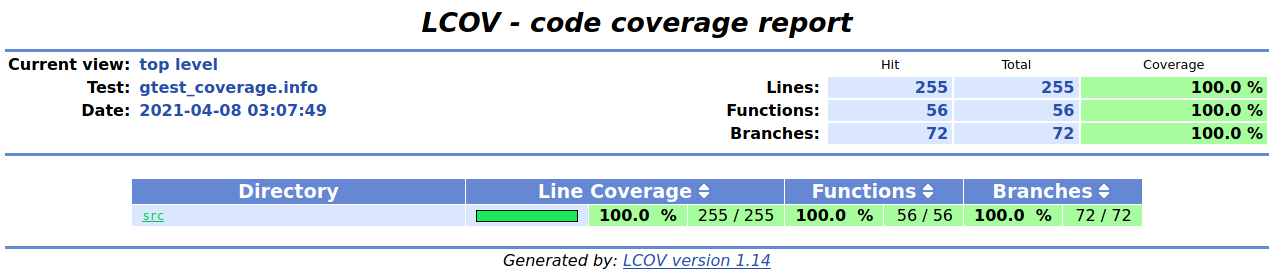
\includegraphics[width=5in]{lcov_ui.png}}
\centerline{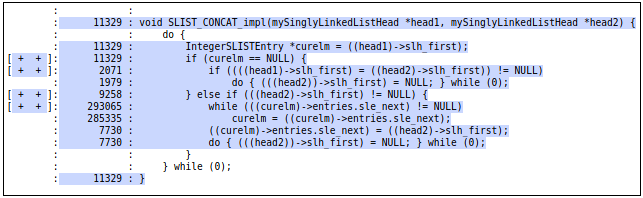
\includegraphics[width=5in]{lcov.png}}
\caption{Visualization of Coverage Metrics Using lcov}
\label{fig:lcov}
\end{figure}

\subsection{Model}

With the tests in place, it was time for the creation of the TLA+ model. The model was split into two modules named LinkedList and Main. LinkedList describes the data structure itself, the structure of the data and the operations that are permitted to be performed on it. Main contains the model checking algorithm verifying that the model works for each possible state,  as well as the invariants verifying that the structure of the linked list holds for each state of the algorithm.

TLA+ almost entirely consists of mathematical sets and functions. Therefore, inspired by the linked list implementation in the book Practical TLA+ \cite{PRACTICALTLA}, was the linked list in this implementation defined as a function. It has a domain of a set of labels, which could be a pointer or a reference in a source code implementation, where each domain entry represents a node in the linked list. The range of the function consists of a function with a finite domain with the labels next and value representing the variables stored in each node (see figure \ref{fig:linkedlists}). 


\begin{figure}[H]
 \vspace{12pt}
\begin{verbatim}
          [NULL |-> [next |-> NULL, value |-> NULL]]
        
          [label1 |-> [next |-> NULL, value |-> INT], 
           label2 |-> [next |-> label1, value |-> INT],
           label3 |-> [next |-> label2, value |-> INT]]
\end{verbatim}
    \centering
    \caption{Linked List Examples}
    \label{fig:linkedlists}
\end{figure}


The label “next” maps to some other label in the linked list domain, indicating that it is the element following the current of the list, or NULL, indicating that the current node is the last. The “value” label maps to some integer held by each node, which in the target source code could be any arbitrary primitive data type or structure.

To check that a function is a valid linked list, a TLA+ operator called IsLinkedList was created (see figure \ref{fig:islinkedlist}). It takes a function as argument, named PointerMap, and checks that for each element in the domain of the PointerMap - NULL included and the label of the first element of the list excluded - there exists a node with the next value representing each node in the function. If that is the case it returns true and false if not. Based on this definition, lists containing cycles are also excluded.

\begin{figure}[H]
 \vspace{12pt}
\begin{verbatim}
        IsLinkedList(PointerMap) ==
            \A el \in ((DOMAIN PointerMap \union {NULL}) \ 
            {First(PointerMap)}): \E x \in DOMAIN PointerMap:
            PointerMap[x]["next"] = el  /\ el /= x
\end{verbatim}
    
    \caption{IsLinkedList Operator}
    \label{fig:islinkedlist}
\end{figure}


As a part of creating arbitrary lists for usage during the model checking process, an operator called PointerMaps was created. It creates a set of functions by mapping from a domain of unique labels it receives as argument to a range (see figure \ref{fig:pointermaps}). PointerMaps creates with this every possible permutation of the domain mapping to every possible permutation of the next range. This means that PointerMaps creates a set of functions that include all valid lists, but also mappings which are not valid.

\begin{figure}[H]
\vspace{12pt}
\begin{verbatim}
    PointerMaps(domain) == 
        [domain -> [value: VALUE, next: domain \union {NULL}]]
\end{verbatim}
    \caption{PointerMaps Operator}
    \label{fig:pointermaps}
\end{figure}


PointerMaps, in combination with IslinkedList, is used in an operator called LinkedList which filters the output from PointerMaps by choosing one of the mappings that IsLinkedList validates as a LinkedList (see figure \ref{fig:linkedlist}). This list, represented as the variable pm, is then returned to be used in the model checking algorithm. If LinkedList on the other hand receives an empty set of domain labels, it returns the representation of an empty list. The empty list is a special case, where NULL is allowed as the only value in the domain of the list (see figure \ref{fig:linkedlists}).

\begin{figure}[H]
\begin{verbatim}
      LinkedList(domain) == 
          IF NULL \in domain 
              THEN Assert(FALSE, "Null cannot be in domain") 
          ELSE IF domain \subseteq {}
              THEN EmptyList
          ELSE
              CHOOSE pm \in PointerMaps(domain):
              IsLinkedList(pm)
\end{verbatim}
    \caption{LinkedList Operator}
    \label{fig:linkedlist}
\end{figure}


With the definition and the ability to create linked lists in place, the concatenation function was added to the model (see figure \ref{fig:concatenation}). It was accomplished via a TLA+ operator taking two lists as arguments and checks if either of the lists are empty. If that is the case, it returns the lists in a TLA+ sequence specified with $<$$<$ $>$$>$, where the empty list is placed at the second index of the sequence. A TLA+ sequence is another way of representing a function where the index of the sequence is equivalent to the domain of a function. It is used in this case to enable the operator to return two lists in a specified order to enable usage using the model checking process (see figure \ref{fig:pluscalconcat}). If both lists are populated there is the special situation where the next value of the last element of the first list needs to be mutated. This is needed since the last element of a list always points to a NULL value and instead needs to show the label of the first element in the second list for them to be considered concatenated.

\begin{figure}[H]
 \vspace{12pt}
\begin{verbatim}
    Concat(list, list2) ==
        IF Empty(list) THEN
            <<list2, list>>
        ELSE IF Empty(list2) THEN
            <<list, list2>>
        ELSE
            LET newLast ==
                CHOOSE x \in [{Last(list)} -> 
                    [value: VALUE, next: {First(list2)}]]:TRUE
            IN
            <<(newLast @@ list) @@ list2, EmptyList>>
\end{verbatim}
    \caption{Concatenation Operator}
    \label{fig:concatenation}
\end{figure}

The concatenation operator is called in the model’s PlusCal algorithm (see TLA+ Tools section \ref{tools}). The concatenation steps consist of a set of labels - PRECONCAT and CONCAT -  with its associated operations (see figure \ref{fig:pluscalconcat}). In PlusCal, the code in each label is disjunct, meaning that each one is a discrete step between which time can progress, and after which the algorithm can stop. Conversely, the code in one label is seen as an atomic unit of progress that cannot be divided further. For this reason, labels must be inserted when, for example, mutating a variable twice. 

\begin{figure}[H]
 \vspace{12pt}
\begin{verbatim}
            PRECONCAT:
            with size \in 0..1 do
            list2 := LinkedList(NewDomain(size, list));
            end with;            
                    
            CONCAT:  
            temp := Concat(list, list2);
            list := temp[1];
            list2:= temp[2];
\end{verbatim} 
    \caption{Concatenation PlusCal Code}
    \label{fig:pluscalconcat}
\end{figure}

All operations under the same label have an associative property meaning that they can be performed in any order. Dividing the operations between labels thereby ensures that the steps of the algorithm are performed in the order intended. PRECONCAT uses the “with” behavior which instructs the model to run the algorithm within the with clause, with every value in the set it is provided – in this case the values 0 and 1. This enables the model checker to perform concatenation operations with all the list sizes to the model's main list variable. The call to the concatenation operator is made under the CONCAT label and stores the returned sequence in the temp variable. From there is then the returned concatenated list - index 1 of the returned sequence - stored in the \textit{list} variable and the returned empty list – index 2 - is stored in the \textit{list2} variable. For every step of the algorithm, the assumptions made about the outcome of the concatenation operator were checked to hold true. This is accomplished through an invariant; a property of a mathematical object which remains unchanged after operations or transformations have been applied to an object of interest (see figure \ref{fig:concatenateinvariant}). This means that they verify for each state that the linked list structure stays valid through the entire model checking phase.

\begin{figure}[H]
 \vspace{12pt}
\begin{verbatim}
ConcatInvariant == 
    IF Empty(list) THEN Concat(list, list2)[1] = list2 
         /\ Empty(Concat(list, list2)[2]) 
    ELSE IF Empty(list2) THEN Concat(list2, list)[1] = list 
         /\ Empty(Concat(list2, list)[2])
    ELSE /\ DOMAIN list \subseteq DOMAIN Concat(list, list2)[1] 
         /\ Empty(Concat(list, list2)[2])
         /\ DOMAIN list \subseteq DOMAIN Concat(list2, list)[1] 
         /\ Empty(Concat(list2, list)[2])
         /\ DOMAIN list2 \subseteq DOMAIN Concat(list, list2)[1] 
         /\ DOMAIN list2 \subseteq DOMAIN Concat(list2, list)[1]
\end{verbatim} 
    \caption{Concatenation Invariant}
    \label{fig:concatenateinvariant}
\end{figure}

Several other invariant operators were also implemented (see figure \ref{fig:invariants}). In the case of this model were they based on the properties established on the list structure such as the list should always be either empty or have a first and last element etc.

\begin{figure}[H]
\begin{verbatim}
        HasFirst == 
            Empty(list) \/ 
            \E el \in DOMAIN list: First(list) = el /\ 
            First(list) \notin Range(list)
        
        HasLast == 
            Empty(list) \/ 
            \E el \in DOMAIN list: list[el]["next"] = NULL 
        
        NullNotInDomain == 
            Empty(list) \/ NULL \notin DOMAIN list
\end{verbatim} 

    \caption{Some Model Invariants}
    \label{fig:invariants}
\end{figure}

Lastly, since the state was written in PlusCal, it was translated by the TLA+ toolbox into pure TLA+ (see figure \ref{fig:puretla}). This is necessary since the model checker can only work with pure TLA+.

\begin{figure}[H]
 \vspace{12pt}
\begin{verbatim}
    PRECONCAT == 
        /\ pc = "PRECONCAT"
        /\ \E size \in 0..1:
           list2' = LinkedList(NewDomain(size, list))
        /\ pc' = "CONCAT"
        /\ UNCHANGED << depth, index, i, from, list, temp,
           arg, lab >>
    
    CONCAT == 
        /\ pc = "CONCAT"
        /\ temp' = Concat(list, list2)
        /\ list' = temp'[1]
        /\ list2' = temp'[2]
        /\ pc' = "INCREMENT"
        /\ UNCHANGED << depth, index, i, from, arg, lab >>
\end{verbatim} 
    \caption{Concatenation State In Pure TLA+}
    \label{fig:puretla}
\end{figure}


\subsection{Reimplementation}

Initially when discussing the details of the reimplementation, it was decided that two versions of the port should be made - one unsafe and one safe (see section \ref{rust}). This was due to some apprehension regarding what was possible to do in safe Rust, and if a linked list could be implemented with the limitations safe Rust brings. If possible, would both versions utilize safe Rust, but not being restricted in one of them could lead to different and interesting model interpretations. 

\subsubsection{Unsafe Version}

The unsafe version was made to match the C-style usage more closely, and references to nodes could be passed to the functions and mutated in place. To achieve this, the nodes were wrapped in a Box type - a type of smart pointer (see line 4 figure \ref{fig:unsafestructs}) \cite{CPPHISTORY}. By wrapping nodes in these smart pointers, the problem of infinitely recursive types as well as other issues were solved. Working with references in general also removes some of the constraints which otherwise would be necessary to put on the concrete type used for the list values, e.g., the clone and/or copy traits. The node struct is used in the linked list structure which stores the head variable representing the first node of the list (see line 8 in figure \ref{fig:unsafestructs}).

\begin{figure}[H]
 \vspace{12pt}
\begin{lstlisting}[style=RUSTSTYLE]
pub trait LinkedListValue: Debug {}
pub struct Node<T: LinkedListValue> {
    pub value: T,
    pub next: Option<Box<Node<T>>>
}

pub struct LinkedList<T: LinkedListValue> {
    pub head: Option<Node<T>>
}
\end{lstlisting} 
    \caption{Unsafe Data Structures}
    \label{fig:unsafestructs}
\end{figure}


Working with boxed references in Rust is like working with references or pointers in C or C++, but with explicit function calls for getting access to the reference - either immutably or mutably. However, unlike a reference in C++, it is not allowed to have both a mutable and immutable reference to an object at the same time, and no two mutable references may refer to the same object, with some exceptions (see section \ref{rust}). As well as using the Box type, it should also be noted that the concept of NULL is not often used in Rust and the consensus is to avoid NULL-pointers at all costs \cite{THERUSTPROGRAMMINGLANGUAGE}. Instead, values which could be NULL-like are wrapped in the Option type, where a value of None represents the NULL case.

Since a TDD methodology was used for the reimplementation, the tests for the unsafe version were then implemented. Every test written was directly based on some invariant or property defined by the model (see figure \ref{fig:correspond} for concatenate example). Several of the hypotheses formed earlier and verified using tests could be combined into a single invariant checking many things, and in the end a single test case in the reimplementation.


\begin{figure}[H]
 \vspace{12pt}
\begin{center}
 \begin{tabularx}{\textwidth}{||X|c|c||}
 \hline
 Target Source Code Test & Model Invariant & Rust Test\\ [0.5ex] 
 \hline\hline
  concatenatingListsEmptiesSecondList & ConcatInvariant & prop\_concat \\ \hline
  concatenatingListsMakesHeadALast-NextHeadBFirst & ConcatInvariant & prop\_concat \\ \hline 
  concatenatingListsYieldsCorrectSizeOn-List1 & ConcatInvariant & prop\_concat \\ \hline
  concatenatingWithHead1EmptyPuts-HeadAFirstOnHeadB & ConcatInvariant & prop\_concat \\ \hline
  concatenatingWithHeadBEmptyPuts-HeadAFirstOnHeadA & ConcatInvariant & prop\_concat \\ \hline
  concatenatingListsPreservesOrder & ConcatInvariant & prop\_concat \\ 
 \hline
\end{tabularx}
\end{center}
    \caption{Tests Corresponding to Concatenation Invariant}
    \label{fig:correspond}
\end{figure}

To continue the concatenation example, a test was implemented verifying that the sizes of the lists after the concatenation operation were correct (see figure \ref{fig:unsafetest}). The test function receives two vectors as argument (line 1). These vectors are used to create lists through the function \textit{linked\_list\_from}, which creates lists with equivalent values as the vector arguments (lines 2 and 3). These lists are then concatenated followed by asserting that the \textit{linked\_list\_2} variable is empty and that size of the \textit{linked\_list\_1} variable corresponds to the sum of the size of the two vector arguments (lines 6 to 9 ). It is also asserted that the concatenated list, the \textit{linked\_list\_1} variable, is of the same size as the sum of the length of the two received vector arguments (line 10). To verify that the values stored in the concatenated list are correct, it is lastly iterated through, and each value compared to those stored in the vectors (lines 13-24). Just as in the original C tests, property-based tests were used through RapidCheck.


\begin{figure}[H]
 \vspace{12pt}
\begin{lstlisting}[style=RUSTSTYLE]
fn prop_concat(list_1: Vec<i32>, list_2: Vec<i32>) -> bool {
    
    let mut linked_list_1 = linked_list_from(&list_1);
    let mut linked_list_2 = linked_list_from(&list_2);
    LinkedList::concat(&mut linked_list_1, &mut linked_list_2);
        
    if linked_list_2.size() != 0 || 
         linked_list_1.size() != list_1.len() + list_2.len() {
         return false;
    }
        
    let mut i = 0;
    for x in linked_list_1.iter() {
        if i < list_1.len() {
            if *x != list_1[i] {
                return false;
            }
        } else {
            if *x != list_2[i-list_1.len()] {
                return false;
            }
        }
        i += 1;
    }
    true
}
\end{lstlisting}
    \caption{Unsafe Size Test}
    \label{fig:unsafetest}
\end{figure}

The concatenation functionality was then implemented in accordance with the tests (see figure \ref{fig:unsafeconcat}). The function receives two linked list arguments (line 2). If the first one has some nodes stored, it iterates through the list to reach the last one (lines 4-9). It then checks if the second list is populated by performing a pattern matching (line 11). If the list is populated then the head of that list is attached to the previously reached last element of the first list (line 12). If on the other hand the first list is empty, then the head of the second list is moved to that empty first list (line 17). This makes the content of the second list being moved to the first while simultaneously asserting that the second list becomes empty.


\begin{figure}[H]
 \vspace{12pt}
\begin{lstlisting}[style=RUSTSTYLE]
pub fn concat(
list_1: &mut LinkedList<T>, list_2: &mut LinkedList<T>) {

    if let Some(head_1) = &mut list_1.head {
        let mut current = &mut head_1.next; 
    
        while let Some(c) = current {
            current = &mut c.next; 
        }
    
        match &list_2.head {
            Some(_) => *current = Some(Box::new(list_2.head.
            take().unwrap())),
            None => {}
        }
    } else {
        *&mut list_1.head = list_2.head.take();
    }
}
\end{lstlisting} 
    \caption{Unsafe Concatenation Function}
    \label{fig:unsafeconcat}
\end{figure}

In line 17 figure \ref{fig:unsafeconcat}, the function \textit{take} is used. When \textit{take} is called on an Option type, the object it is called upon becomes None, and a new Option containing the value is returned. This essentially moves the value from one Option to another in place \cite{RUSTMANUAL}, in this case appending the head of one list onto the tail of another.

In the cases where an immutable reference to an object was needed, but only needed for equality checks - i.e., never read from - this was solved by using the address of the object in question instead of a reference to it. This is both safe and mitigates the issues working directly with references would cause. The implementation of the insert before function (see figure \ref{fig:insertbefore}), which takes the address of a node and a value to insert, serves as an example of this.

\begin{figure}[H]
 \vspace{12pt}
\begin{lstlisting}[style=RUSTSTYLE]
pub fn insert_before(&mut self, node: *const Node<T>, value: T) {
    if self.head.is_some() {
        let head = self.head.as_mut().unwrap();
        if node == head as *const _ {
            self.insert_head(value);
        } else
        {
            head.insert_before(node, value);
        } 
    } else {
        panic!("Cannot insert into empty list");
    }
}
\end{lstlisting}
    \caption{Insert Before}
    \label{fig:insertbefore}
\end{figure}

If a reference was used to identify the node to insert before, the signature would have been valid but very difficult to use. That is, since the list would have a reference to the node, which would also be passed a reference to the function, this usage is disallowed by the borrow checker. As a work-around, something like what can be seen in figure \ref{fig:unsafehelper} would have been needed. Working directly with addresses only works when there is some guarantee that the node itself will never unexpectedly move around in memory. Since the node does not implement either copy or clone, this holds for all cases except where the user explicitly moved it.

\begin{figure}[H]
 \vspace{12pt}
\begin{lstlisting}[style=RUSTSTYLE]
pub fn create_unsafe_ref<T>(node: &Node<T>) -> Option<&Node<T>> {
    let mut return_node: Option<&Node<T>> = None;
    unsafe { 
        return node = Some(&*node as *const _);
    }
    return_node
}
\end{lstlisting}
    \caption{Unsafe Helper Function}
    \label{fig:unsafehelper}
\end{figure}


The signature for \textit{insert\_before} could then instead be as in figure \ref{fig:insertbeforesignature}. In the end it should be noted that even though there were initially thought that unsafe code would be necessary to implement the functionality using reference, unsafe was not necessary.

\begin{figure}[H]
 \vspace{12pt}
\begin{lstlisting}[style=RUSTSTYLE]
    pub fn insert_before(&mut self, node: &Node<T>, value: T)
    ...
\end{lstlisting}
    \caption{Insert Before With References}
    \label{fig:insertbeforesignature}
\end{figure}


\subsubsection{Safe Version}

The safe version was implemented through a structure consisting of several fields. The "nodes" field is a vector holding each node located on the list (see line 10 in figure \ref{fig:safestructures}). The "head" field stores the vector index position of the first node of the list (line 11) and the "size" field indicates how many nodes the list currently consists of (line 12). To know which indexes of the nodes vector - if any - are free due to nodes having been removed from the list a stack called "freeindex" is also stored (line 13). The node structure stores the value of the vector index it is located on in contrast to what position it has in the list (line 4). It also stores the vector index of the node which follows it in the list in its "next" field (line 5) and has a "value" field for node value storage as well (line 6). As opposed to the unsafe version, the idea here is to work with copies of the nodes rather than references. These copies are then used by the list similarly as if they are references, but with the difference that the user cannot change the structure of the list without calling predefined methods.

\begin{figure}[H]
 \vspace{12pt}
\begin{lstlisting}[style=RUSTSTYLE]
pub trait LinkedListValue: Copy + Clone {}
#[derive(Copy, Clone)]
pub struct Node<T: LinkedListValue> {
    index: usize, 
    next: Option<usize>,
    pub value: T
}

pub struct LinkedList<T: LinkedListValue> {
    nodes: Vec<Node<T>>,
    head: Option<usize>,
    size: usize,
    freeindex: Vec<usize>
}
\end{lstlisting}
    \caption{Safe Data Structures}
    \label{fig:safestructures}
\end{figure}

\newpage

The safe test has many similarities to the unsafe version where it receives two vector arguments of arbitrary sizes and values (see line 1 figure \ref{fig:safetest}), used to create two lists which get concatenated. The sizes of the lists are then asserted followed by the concatenated list being iterated through to check that the values are correct.

\begin{figure}[H]
 \vspace{12pt}
\begin{lstlisting}[style=RUSTSTYLE]
fn prop_concat(list_1: Vec<i32>, list_2: Vec<i32>) -> bool {
    let mut linked_list_1 = linked_list_from(&list_1);
    let mut linked_list_2 = linked_list_from(&list_2);
    
    match LinkedList::concat(&mut linked_list_1, 
    &mut linked_list_2) 
    {
        Ok(_) => {
            if linked_list_2.size() != 0 || 
            linked_list_1.size() != list_1.len() + list_2.len() {
                return false;
            }
            
            let mut i = 0;
            for x in linked_list_1.iter() {
                if i < list_1.len() {
                    if x != list_1[i] {
                        return false;
                    }
                } else {
                    if x != list_2[i-list_1.len()] {
                        return false;
                    }
                }
                i += 1;
            }
            true
        },
        _ => false
    }
}
\end{lstlisting}
    \caption{Safe Test}
    \label{fig:safetest}
\end{figure}

The safe reimplementation of the concatenation operation takes two lists as arguments (see line 1 figure \ref{fig:safeconcat}). If the second list is not populated, the function simply returns since in this case it is irrelevant if the first list is populated or not (lines 4-6). If the second list is populated and the first list is empty however, \textit{mem::swap} is used (lines 8-11). This swaps the memory contents of the lists which provides the intended functionality of moving the second list to the first and vice versa. If both lists on the other hand are populated, then the last element of the first list is found by using the helper function \textit{node\_at\_index} (line 13). This function takes the list position of the node of interest as argument and iterates through the list until it has reached the node in question and returns it. The head of the second list is then inserted after this node (lines 23-26). A procedure accomplished by using the \textit{insert\_after} function which takes a node and a value as argument and creates a new node with said value and inserts it after the received node. The head then lastly is removed to remove the node from the second list (lines 27-31). When this procedure of insertion and removal has been performed for each element of the second list, the lists are concatenated and an Ok result is returned (line 34).

\begin{figure}[H]
 \vspace{12pt}
\begin{lstlisting}[style=RUSTSTYLE]
pub fn concat(list_1: &mut Self, list_2: &mut Self) -> 
LinkedListResult<()>  {
    
    if list_2.is_empty() {
        return Ok(());
    }

    if list_1.is_empty() {
        mem::swap(list_1, list_2);
        return Ok(());
    }

    let mut list_1_end = match list_1.node_at_index(
    list_1.size()-1) {
        Ok(Some(node)) => node,
        Ok(None) => {
            mem::swap(list_1, list_2);
            return Ok(())
        },
        Err(e) => return Err(e) 
    };
        
    while let Some(next) = list_2.head() {
        if let Ok(new_end) = list_1.insert_after(
        list_1_end, next.value) {
            list_1_end = new_end; 
            match list_2.remove_head() {
                Ok(_) => {},
                    _ => return Err(LinkedListError{message:
                    String::from("Error concatenating lists")})
                }
            }
        }
    Ok(())
}
\end{lstlisting}
    \caption{Safe Concatenation Implementation}
    \label{fig:safeconcat}
\end{figure}


\subsection{Verification}


To reliably verify the result, the two ports were - as well as the original code - wrapped in a common API (see figure \ref{fig:agnosticapi}). Each version was built as a library and linked into the test program. The common interface always returns an unsigned integer where negative values means that an error occurred. The library calls were wrapped in implementations of a \textit{LinkedListLib} class - \textit{Clib} and \textit{RustLib} - which were responsible for calling the correct library functions. This helped in making the libraries easily interchangeable (lines 4 and 10). 

As Rust has no stable API for C++, the interface was called from C, although other parts of the test code were written in C++. The intention was to reuse the original property-based tests with the two linkable libraries. To call Rust code from C, headers specifying the library interface must be created. No tool that does this is directly available in the common rust build tools, but the community provides a tool called cbindgen to do this automatically \cite{CBINDGEN}.

\begin{figure}[H]
 \vspace{12pt}
\begin{lstlisting}[style=CSTYLE]
int32_t Clib::concatenate(
uintptr_t identifier_list_1, 
uintptr_t identifier_list_2) {
    return clib_concatenate(identifier_list_1, identifier_list_2);
}

int32_t RustLib::concatenate(
uintptr_t identifier_list_1, 
uintptr_t identifier_list_2) {
    return rlib_concatenate(identifier_list_1, identifier_list_2);
}
\end{lstlisting}
    \caption{Agnostic Test APIs}
    \label{fig:agnosticapi}
\end{figure}

An example of how this interface works is the concatenate call (see figure \ref{fig:agnostichelper}). It returns zero if no error occurs (lines 7 and 17), otherwise another integer value representing an error-code is returned (line 21). The library is in control of the memory allocations for, and the managing of the lists. A call to the library can create a new or modify an existing list. When creating a list, the library returned a unique identifier corresponding to that list. All other functions represented either a modification to an existing list, or a getter for a value from the list or some property of the list. These functions take one or more list identifiers and optionally some value and/or index. The libraries were then subjected to property-testing. The original test suite could be reused, although with slight modification to work with the list libraries. 

\begin{figure}[H]
 \vspace{12pt}
\begin{lstlisting}[style=CSTYLE]
int32_t clib_concatenate(
uintptr_t identifier_list_1, 
uintptr_t identifier_list_2) {
    auto head_1 = lists.at(identifier_list_1);
    auto head_2 = lists.at(identifier_list_2);
    SLIST_CONCAT_impl(head_1, head_2);
    return 0;
}

pub extern "C" fn rlib_concatenate(
identifier_list_1: usize, 
identifier_list_2: usize) -> i32 {
    let mut lists = LISTS.lock().unwrap();
    if let (Some(list_1), Some(list_2)) = 
    lists.borrow_two(identifier_list_1, identifier_list_2) {
        match LinkedList::concat(list_1, list_2) {
        Ok => 0,
        _ => -1
        }
    } else {
        -1
    }
}
\end{lstlisting}
    \caption{FFI Interface Concatenate Functions}
    \label{fig:agnostichelper}
\end{figure}